
% This LaTeX was auto-generated from MATLAB code.
% To make changes, update the MATLAB code and republish this document.

\documentclass{article}
\usepackage{graphicx}
\usepackage{color}

\sloppy
\definecolor{lightgray}{gray}{0.5}
\setlength{\parindent}{0pt}

\begin{document}

\title{Deber 2, Se\~nales y Sistemas}
\author{Camilo Acosta}
\maketitle

    
    \begin{verbatim}
function [ ] = ejercicio1(  )
%Universidad de las Fuerzas Armadas
%Autor: Camilo Acosta
%Senales y Sistemas
%Deber 2 Convolucion en Matlab

%El sistema que se muestra en la siguiente figura esta formado con la
%conexion de dos sistemas en cascada. Las respuestas al impulso de los
%sistemas son:


%h1[n]=(1/6)^(n-6)*u[n]%
%h2[n]=(1/3)^(n)*u[n-3]%


%Se procede a hallar h3[n] por medio de la conexion en serie del sistema
%LTI1 con el LTI2, al ser en serie el h3[n] es el resultado de la
%convolucion de h1[n] con h2[n].

%se limpia todas las variables del Workspace
clear all
%Se cierran todas las figuras
close all
%Para crear la primera senal discreta se crea un vector n que la delimite
n=0:1:10;
%Dada la funcion Escalon definida por:
%......................................
%function [ h ] = escalon( n )
%h = n>=0;
%end
%......................................

%Usando la funcion escalon se crea una funcion h1[n]:

h1=((1/6).^(n-6)).*(escalon(n));

%Usando stem() se grafica de manera discreta h1[n], de color rojo
stem(n,h1,'r');
grid
xlabel('n')
ylabel('h1[n]')
title('Senal h1[n]')

%Para crear  senal discreta h2[n] se crea un vector n2 que la delimite
n2=0:1:10;


%Se crea la funcion cuadrada a partir del escalon que toma los valores.
%Se desplaza el escalon temporalmente tres muestras a la derecha.

h2=(escalon(n2-3)).*((1/3).^(n2));

%Usando stem() se grafica de manera discreta h2[n], de color verde
figure;
stem(n2,h2,'g');
grid
xlabel('n')
ylabel('h2[n]')
title('Senal h2[n]')

%Se obtiene la convolucion usando conv()
h3=conv(h1,h2);
figure
%n3=n+n2-1
%para saber la longitud de n3 solo basta con -2 al limite superior de n3
%para que matlab entienda. No es necesario sumar nada mas porque ambas
%senales x[n] y h[n] empiezan despues de cero
n3=0:1:length(h1)+length(h2)-2;
%Usando stem() se grafica de manera discreta y[n], usando n3
stem(n3,h3);
grid
xlabel('n')
ylabel('h3[n]')
title('Senal h3[n]')

end
\end{verbatim}

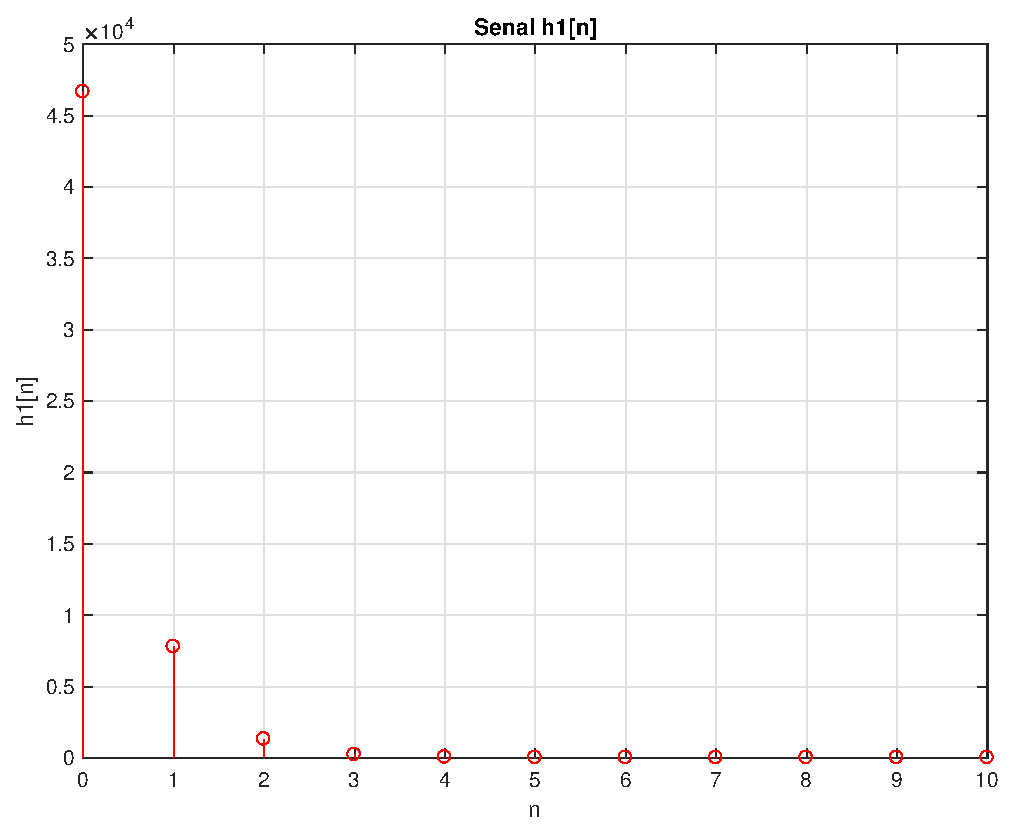
\includegraphics [width=4in]{ejercicio1_01.eps}

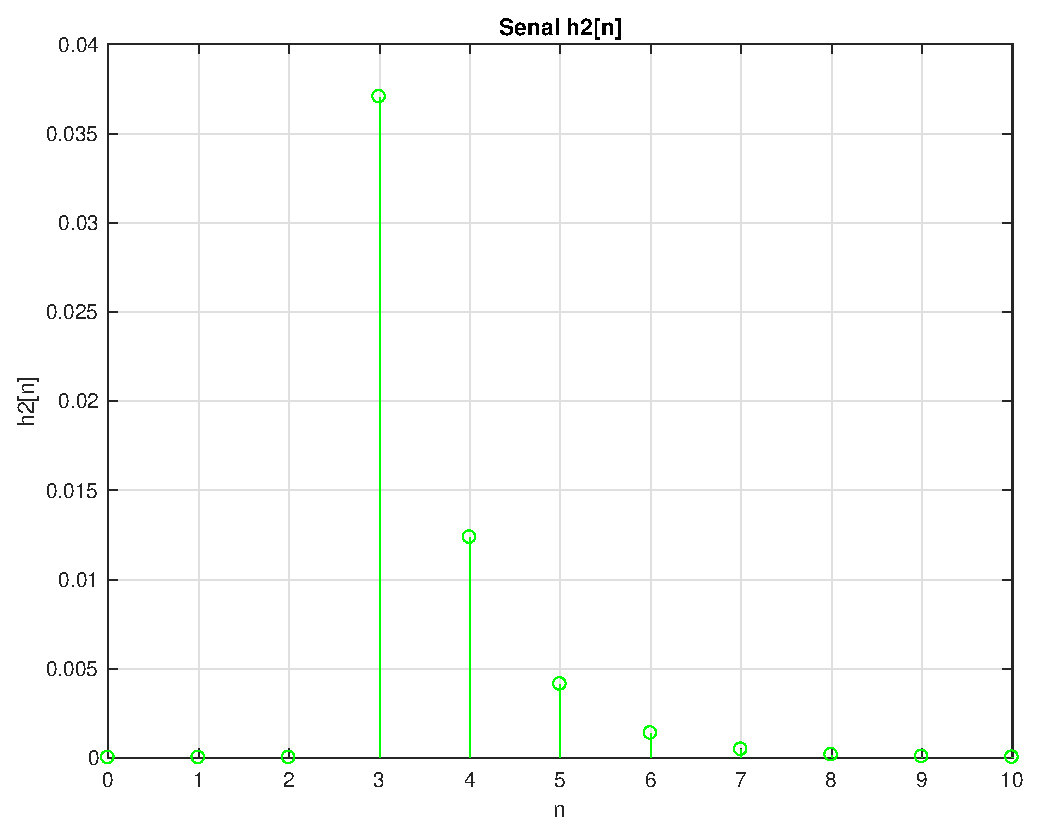
\includegraphics [width=4in]{ejercicio1_02.eps}

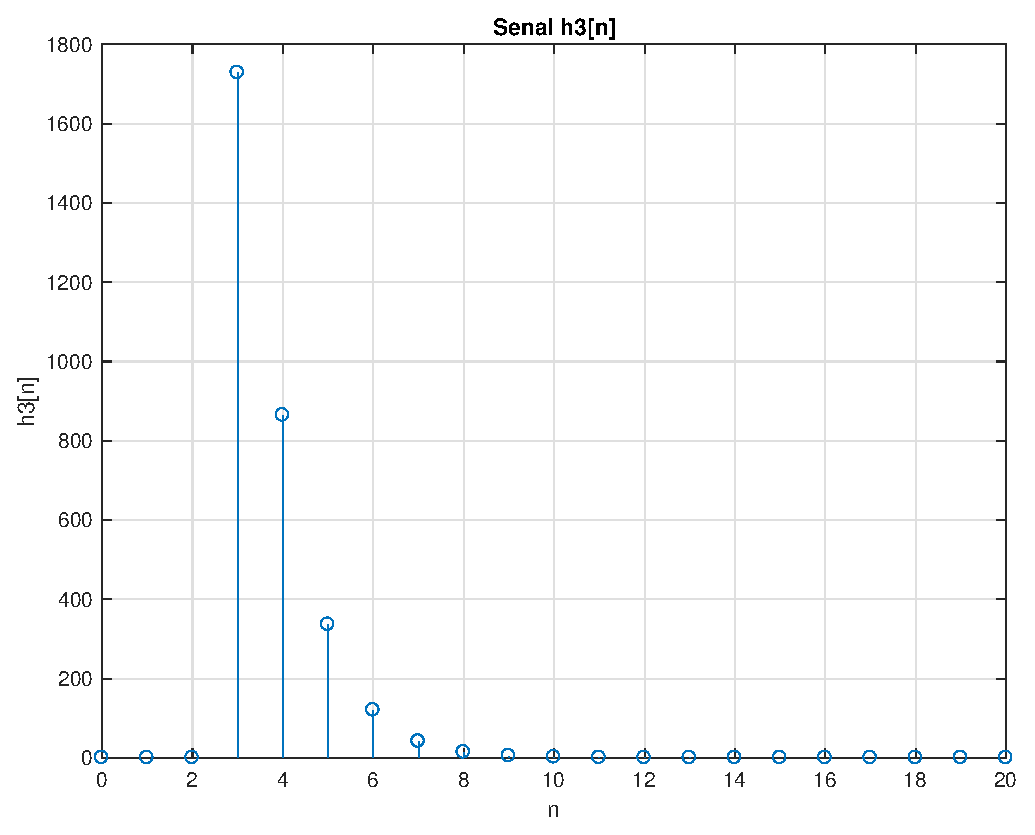
\includegraphics [width=4in]{ejercicio1_03.eps}


    \begin{verbatim}
function [ ] = ejercicio_2(  )
%Universidad de las Fuerzas Armadas
%Autor: Camilo Acosta
%Senales y Sistemas
%Deber 2 Convolucion en Matlab

%Dada la respuesta al impulso de un sistema LTI, h(t)=u(t-1)-u(t-4).
%Encuentra la salida del sistema en respuesta a la entrada
%x(t)=u(t)+u(t+1)-2u(t-2).

%Se limpia todas las variables del Workspace
clear all
%Se cierran todas las figuras
close all
%Para crear la primera senal discreta se crea un vector t que la delimite
%Se usa intervalos de 0.01 para que parezca una senal continua.
t=0:0.01:10;
%Dada la funcion Escalon definida por:
%......................................
%function [ h ] = escalon( n )
%h = n>=0;
%end
%......................................

%Usando la funcion escalon se crea una funcion "cuadrada" discreta, que va
%usando el vector t

h=(escalon(t-1)-escalon(t-4));

%Usando plot() se grafica de manera 'continua' h(t), de color rojo
plot(t,h,'r');
grid
xlabel('t')
ylabel('h(t)')
title('Senal h(t)')

%Para crear la primera senal discreta se crea un vector t2 que la delimite
%Se usa intervalos de 0.01 para que parezca una senal continua.
t2=-2:0.01:10;

x=escalon(t2+1)+escalon(t2)-2*escalon(t2-2);


%Usando plot() se grafica de manera 'continua' x(t), de color azul
figure;
plot(t2,x,'b');
grid
xlabel('t')
ylabel('x(t)')
title('Senal x(t)')

%Se obtiene la convolucion usando conv()
y=conv(x,h)*0.01;
figure
%El vector t3 delimita al eje temporal
%t3 va en intervalos de 0.01, por lo que a su limite superior
%(length(x)+length(h)-2) se lo multiplica por 0.01
%para saber el limite inferior  y superior del vector t3,  se suma el
%limite inferior del vector t2, que es -2, a ambos limites del vector t3

t3=-2:0.01:((length(x)+length(h)-2)*0.01)-2;
%Usando plot() se grafica de manera 'continua' y(t), usando t3, con el
%color cyan.
plot(t3,y,'cyan');
grid
xlabel('t')
ylabel('y(t)')
title('Senal y(t)')

end
\end{verbatim}

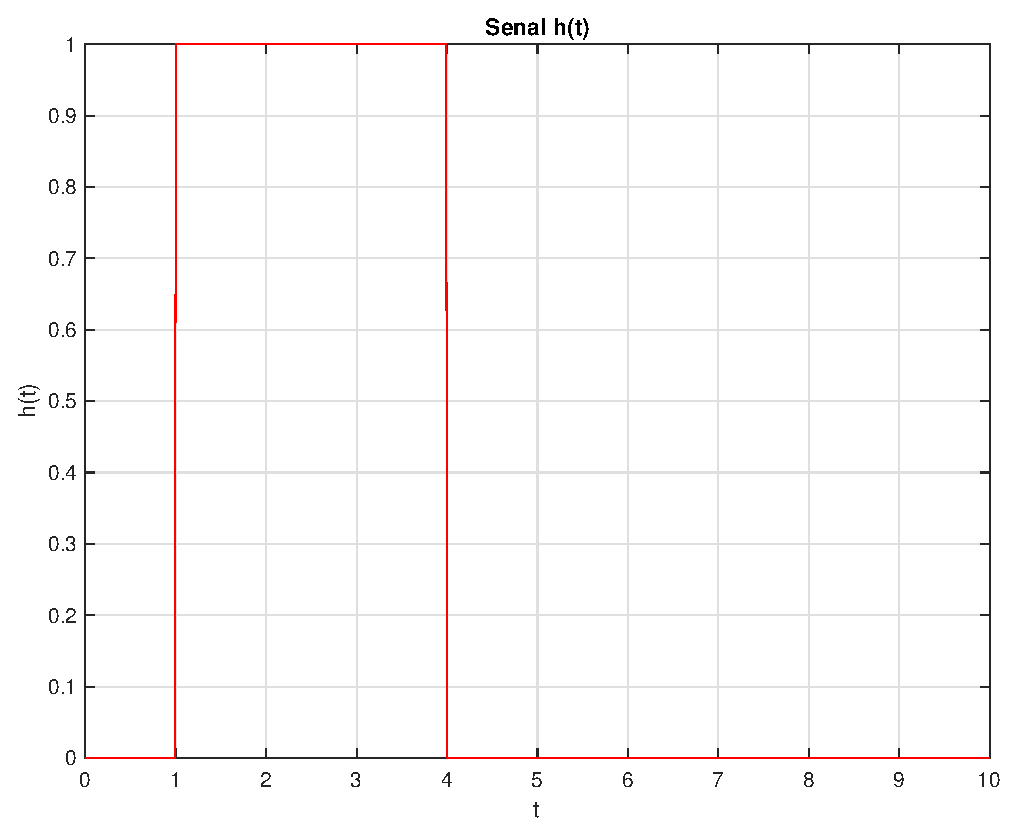
\includegraphics [width=4in]{ejercicio_2_01.eps}

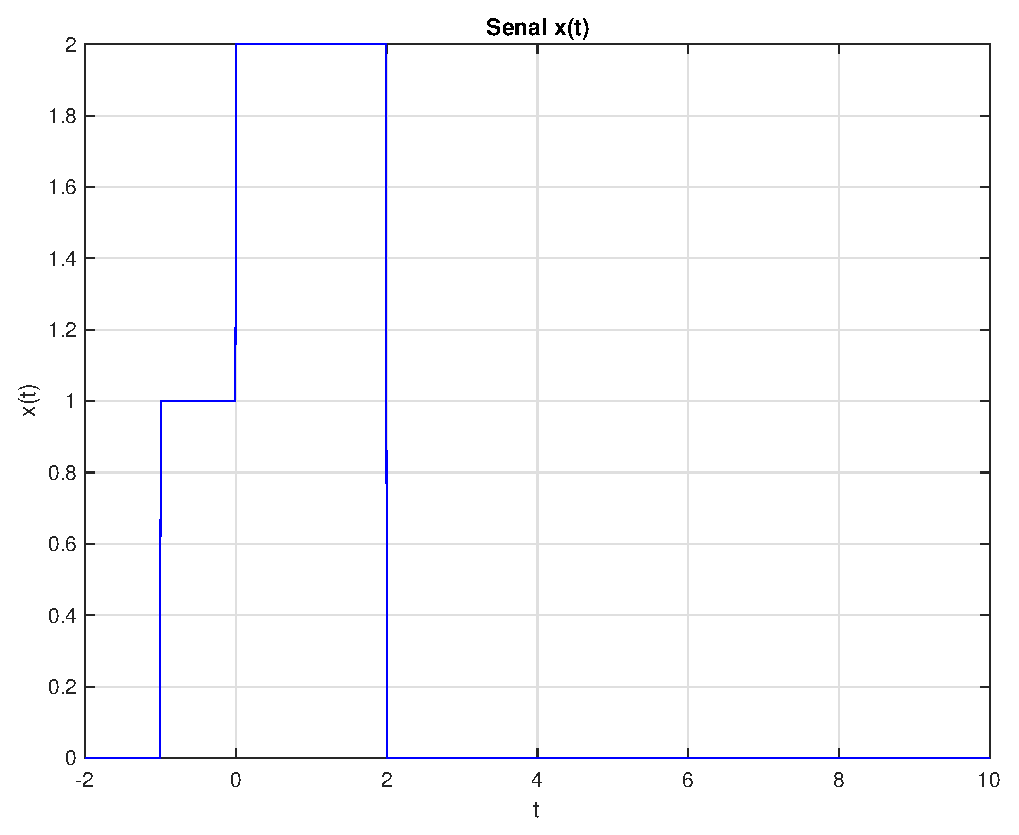
\includegraphics [width=4in]{ejercicio_2_02.eps}

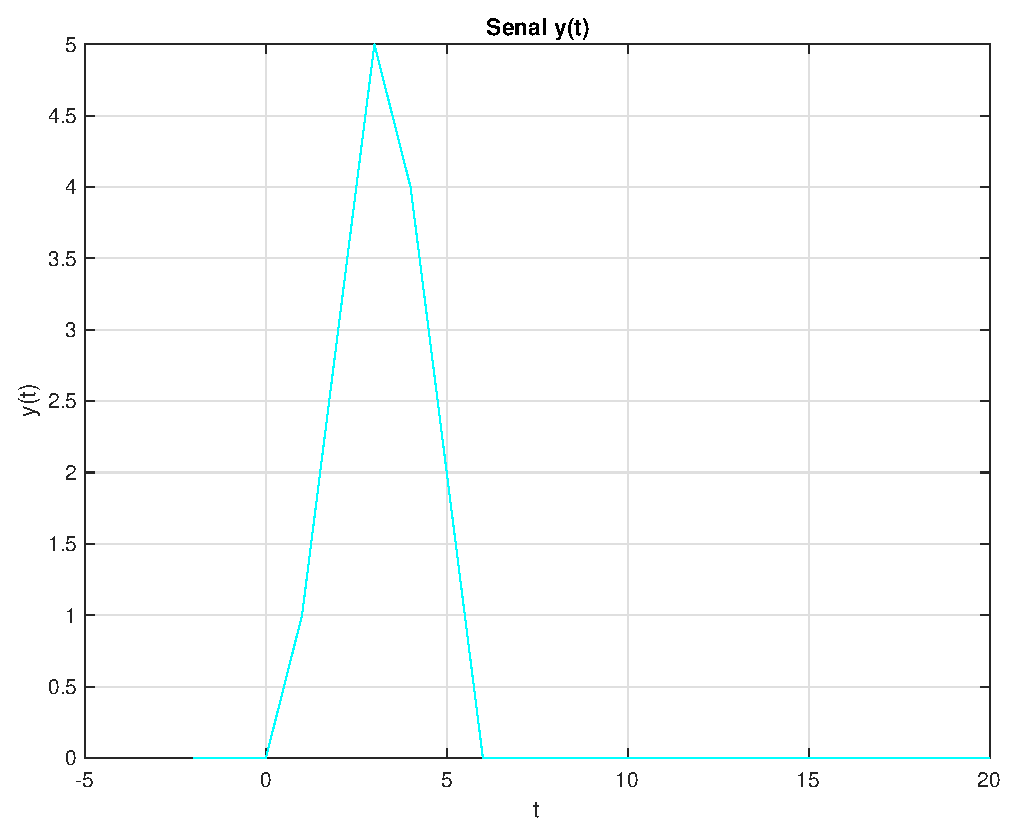
\includegraphics [width=4in]{ejercicio_2_03.eps}



\end{document}
    
